\documentclass[a4paper,11pt]{article}
\usepackage{amsmath,amssymb,amsfonts,latexsym}
\usepackage[utf8]{inputenc}
\usepackage{fancyvrb}
\usepackage{graphicx}
\usepackage[margin=1.1in]{geometry}
\usepackage{url}
\usepackage{verbatim}
\usepackage{fixltx2e}
\usepackage{amsfonts}
\usepackage{amssymb}
\usepackage{amsmath}
\usepackage{float}
\usepackage{listings}
\usepackage{lmodern}
\usepackage[spanish]{babel}
\lstset{frame=tb,
  language=Java,
  aboveskip=3mm,
  belowskip=3mm,
  showstringspaces=false,
  columns=flexible,
  basicstyle={\small\ttfamily},
  numbers=none,
  breaklines=true,
  breakatwhitespace=true
  tabsize=3
}
\providecommand{\keywords}[1]{\textbf{\textit{Palabras clave:}} #1}
\title{Ising Model \\
MVMISG  \\ M\'etodos Num\'ericos Avanzados}
\author{Enzo Altamiranda, Mauricio Minestrelli, Cristian Ontivero, Valeria Serber}
\date{\today}
\begin{document}

\maketitle
\thispagestyle{empty}
\vspace{3cm}

\renewcommand{\abstractname}{Resumen}
\begin{abstract}
%Desarrolle un programa para que, dado m, construya la matriz A. Verifique el correcto funcionamiento de su programa con las matrices que se encuentran en Matrix Market.
%Implemente un programa que calcule num\'ericamente los autovalores de A dado m. ¿Cu\'al es la mayor dimensi\'on de la matriz con la que puede trabajar su programa? Verifique el correcto funcionamiento usando el alg\'un programa matem\'atico como Matlab u Octave.
Se presentan los resultados que se obtuvieron al implementar diferentes
estructuras de datos y algoritmos en C para, dado a partir de un par\'ametro
que define el tamaño de una matriz con origenes en el modelo de Ising,
generarla.  Posteriormente, para evitar los detalles de C se mueve a Octave,
y se muestra un m\'etodo para calcular los autovalores de la misma.\\[5 pt]
\keywords{Matracies ralas, Matrices dispersas, Compressed Column storage,  Compressed sparse column, Modelo de Ising}
\end{abstract}
\section{Introducci\'on}
\begin{comment}
[Introduce el tema contextualizando la informacion. Puede incluirse un parrafo con una breve descripcion historica, otro parrafo motivando el tema. El ultimo parrafo de esta seccion tiene que ser la descripcion de la estructura del artıculo, explicitando en que seccion se trata cada tema.]
\end{comment}
\paragraph{}
El \emph{Modelo de Ising} es un modelo f\'isico utilizado en el estudio del
comportamiento de materiales ferromagn\'eticos, propuesto por el f\'isico
\emph{Wilhelm Lenz} en 1920 a su estudiante \emph{Ernst Ising}, qui\'en
demostr\'o que el modelo unidimensional no ten\'ia transici\'on de fase para su
tesis en 1924. La matriz tratada en el presente trabajo tiene sus or\'igenes en
este modelo, y surge de un producto de matrices que se explicar\'a m\'as
adelante.
\paragraph{}
En este informe se describen las distintas instancias sucedidas en el
desarrollo de un programa que calcula la matriz del \emph{Modelo de Ising},
junto con sus autovalores. Se mencionan los algoritmos elegidos y c\'omo se fue
optimizando los mismos, as\'i como tambi\'en las estructuras utilizadas, con el
objetivo de lograr una menor complejidad en el c\'odigo y una mayor rapidez
para generar resultados. Tambi\'en se muestran las pruebas realizadas y
gr\'aficos que comparan las distintas iteraciones del desarrollo.
\newpage
\section{Metodolog\'ia}
\begin{comment}
[Hay que relatar los pasos que se fueron realizando, incluyendo los modelos utilizados, los analisis hechos, las pruebas realizadas.]
\end{comment}
\subsection{C\'alculo de la matriz del Modelo de Ising}
\paragraph{}
La matriz del Modelo de Ising, llamada \textbf{\emph{A}} a partir de ahora,
puede calcularse como el producto de dos matrices \textbf{\emph{K}} y
\textbf{\emph{L}}, ambas de dimensi\'on \emph{2m} x \emph{2m}, con \emph{m}
perteneciente a los naturales.
% \times para el x, \in para pertenece \mathbb{N} para naturales
\begin{equation} \label{matrizA}
A = K L
\end{equation}
donde
\begin{equation} \label{matrizK}
K =
\left( \begin{array}{ccccc}
E &  &  &  & \\
 & E &  &  & \\
 &  & \ddots &  & \\
 &  &  & E & \\
 &  &  &  & E\end{array} \right),	E =
 \left( \begin{array}{cc}
  \cos \alpha & \sin \alpha\\
-\sin \alpha & \cos \alpha\end{array} \right)
\end{equation}
\\
\begin{equation} \label{matrizL}
L =
\left( \begin{array}{ccccc}
\cos \beta &  &  &  & -\sin \beta\\
 & F &  &  & \\
 &  & \ddots &  & \\
 &  &  & F & \\
\sin \beta &  &  &  & \cos \beta\end{array} \right),	F =
 \left( \begin{array}{cc}
  \cos \beta & \sin \beta\\
-\sin \beta & \cos \beta\end{array} \right)
\end{equation}
\subsubsection{Primera Iteraci\'on}
\paragraph{}
En la primera iteraci\'on se opt\'o por almacenar cada matriz en un arreglo de
arreglos. Se comenz\'o realizando una implementaci\'on del algoritmo est\'andar
de multiplicaci\'on de matrices, debido a la simpleza del c\'odigo
correspondiente. Se prob\'o esta versi\'on creando las matrices \emph{K} y
\emph{L} y multiplic\'andolas. El orden temporal de este algoritmo es c\'ubico,
es decir, \emph{O(n\textsuperscript{3})}. Debido a esto, al calcular matrices
pequeñas el algoritmo termina de forma r\'apida, sin embargo, al probar
matrices de mayor tamaño, el tiempo crece en gran medida.
\subsubsection{Segunda Iteraci\'on}
\paragraph{}
Una vez visto los l\'imites de la implementaci\'on densa, se opt\'o por aprovechar el
hecho de que las matrices necesarias para la construcci\'on de la matriz A,
incluida esta \'ultima, eran todas ralas.  Para optimizar el algoritmo, se
decidi\'o por cambiar la estructura de datos que almacena las matrices, de modo
que los ceros no se almacenen, y el algoritmo de multiplicaci\'on pueda los productos
de valores nulos.

La estructura utilizada en esta iteraci\'on se conoce como \emph{``Compressed
column storage''} \emph{(CCS)}, o alternativamente \emph{``Compressed sparse
column''}, y es la representaci\'on tradicional utilizada en \emph{MATLAB} al
usar la funci\'on \emph{``sparse''}.
\paragraph{}
Esta representaci\'on cuenta con tres arreglos. El primero, al cual llamaremos
\textbf{\emph{values}}, contiene los valores no nulos de la matriz, de tamaño
\textbf{\emph{nnz}} (del ingl\'es \emph{``number of nonzeros''}). El segundo,
\textbf{\emph{r\textsubscript{i}}}, indica el \'indice de la fila del elemento
que se encuentra en el primer arreglo y en la misma posici\'on. Dicho arreglo
tambi\'en tiene tamaño \emph{nnz}. El tercero, \textbf{\emph{cp}}, tiene como
tamaño la cantidad de columnas m\'as uno, donde en la posici\'on \emph{j} del
arreglo se guarda el \'indice en el arreglo de valores, en el que se encuentra
el primer elemento no nulo de la columna \emph{j}. El \'ultimo elemento de
\emph{cp} es el valor \emph{nnz}. Si alguna columna tuviera todos ceros, en el
\'indice de esa columna se coloca el mismo valor que en la pr\'oxima columna.

\textbf{Ejemplo de almacenamiento de una matriz utilizando Compressed column storage}\\
\[ M = \left( \begin{array}{ccccc}
0 & 3 & 0 & 5 & 7 \\
0 & 0 & 0 & 3 & 8 \\
1 & 0 & 0 & 0 & 0 \\
0 & 2 & 0 & 0 & 5\end{array} \right)\]

\paragraph{}
Notar que la tercer columna no tiene valores. Esto se representa usando el
mismo valor en \emph{cp} que en la pr\'oxima columna. Esto es consistente con
el hecho de que la cantidad de elementos no nulos presentes en la columna
\emph{j} se puede conocer con la resta \[\emph{cp[j+1] - cp[j]}.\]

\[ values = \left[ \begin{array}{cccccccc}
1, & 3, & 2, & 5, & 3, & 7, & 8, & 5 \\\end{array} \right]\]

\[ ri = \left[ \begin{array}{cccccccc}
2, & 0, & 3, & 0, & 1, & 0, & 1, & 3 \\\end{array} \right]\]

\[ cp = \left[ \begin{array}{cccccc}
0, & 1, & 3, & 3, & 5, & 8\\\end{array} \right]\]
\\
\textbf{Complejidad espacial de la representaci\'on CCS}
\paragraph{}
Para una \textbf{matriz densa}, es decir, que no tiene elementos nulos, de
\emph{m} x \emph{n}, se necesitan \emph{m} punteros en memoria, cada uno
apuntando a los \emph{m} arreglos de \emph{n} elementos. En comparaci\'on con
una matriz en representaci\'on \emph{CCS}, se necesita espacio para
\emph{nnz$\cdot$sizeof(elementos) + (nnz + cols)$\cdot$sizeof(\'indices)}. Para una
aproximaci\'on m\'as f\'acil de entender, si suponemos que el tamaño de
\'indices, elementos, y punteros en memoria usan todos a misma cantidad de
bytes, se tiene que la complejidad espacial de la matriz densa es
\emph{m+m$\cdot$n}, es decir, \emph{O(m$\cdot$n)}. Como en el caso del Modelo
de Ising las matrices son cuadradas, el orden espacial resulta
\emph{O(n\textsuperscript{2})}. En cambio, la complejidad espacial de la
\textbf{matriz rala} es \emph{2$\cdot$nnz+n}, es decir orden \emph{O(nnz+n)},
el cual es \emph{lineal}.\\
\\
\textbf{Algoritmo de multiplicaci\'on CCS}
\paragraph{}
Al utilizar la representaci\'on \emph{CCS}, se logr\'o un algoritmo de
multiplicaci\'on significativamente m\'as eficiente (como se verá a
continuación), ideal para matrices ralas, ya que bastó con multiplicar y sumar
solamente los valores no nulos de las matrices, ignorando los ceros.
A continuaci\'on se observa en pseudoc\'odigo, el algoritmo implementado para
multiplicar utilizando la estructura \emph{CCS}, que difiere del algoritmo
est\'andar utilizado anteriormente. Cabe destacar que tanto este algoritmo como
la representación CCS de matrices, requieren que las matrices sean efectivamente
dispersas para presentar ventajas ante el algoritmo y estructura tradicional
de matrices densas.\\
\newpage
\small\begin{lstlisting}
CCSMatrix matriz = nueva matriz de m x n;

Por cada columna de la 2da matriz {
    Si la columna no tiene elementos entonces saltearla;

 	Por cada fila de la 1ra matriz {

 		currentVal = suma de los productos de los valores no nulos de la columna actual, con los correspondientes de la fila actual;

		             Si currentVal es cero entonces saltear la fila;

 		Si aun no se registro el valor que comienza la columna actual {

	 		Registrar;

 			Si habia columnas salteadas por no tener elementos entonces propagar el valor actual hacia atras;
		}

 		Almacenar el valor no nulo actual;

 		Almacenar el indice de la fila del valor no nulo actual;
	}
}

Almacenar el numero de valores no nulos en la matriz;

Almacenar el numero de valores no nulos en la posicion final del arreglo de punteros de columnas;

Retornar matriz;

\end{lstlisting}
\small\emph{Algoritmo de multiplicaci\'on CCS: Se muestra en pseudoc\'odigo el
algoritmo que calcula la multiplicaci\'on de las matrices K y L aprovechando la
estructura de datos CCS.}

\newpage
\section{Resultados}
\subsection{Comparaci\'on entre ambas iteraciones}
\paragraph{}
Se realizaron pruebas en ambas iteraciones para descubrir las diferencias entre
ellas. Se utilizaron matrices de diferentes tamaños, y se utiliz\'o el comando
\emph{``time''} de \emph{Linux} para medir el tiempo en cada caso. Para
consistencia y coherencia en los resultados, todas las pruebas se hicieron en
una misma computadora, de procesador Intel Core i7 3612QM 2.1 GHz y 8 GB DDR3
de memoria RAM. A continuaci\'on se muestra una tabla con los valores que se
utilizaron en las pruebas, y luego los gr\'aficos que se realizaron a partir de
ellas.\\
\\

\begin{tabular}{|l||l|l||l|}
\hline
\multicolumn{2}{|l|}{Multiplicaci\'on est\'andar}&\multicolumn{2}{l|}{Multiplicaci\'on CCS}\\
\cline{1-4}
\textbf{m}&\textbf{tiempo (seg)}&\textbf{m}&\textbf{tiempo (seg)}\\
\hline\hline
100 & 0.02 & 100 & 0\\
150 & 0.05 & 150 & 0\\
200 & 0.13 & 200 & 0\\
250 & 0.25 & 250 & 0.01\\
300 & 1.32 & 300 & 0.01\\
350 & 2.88 & 350 & 0.01\\
400 & 4.24 & 400 & 0.01\\
450 & 6.51 & 450 & 0.02\\
500 & 8.90 & 500 & 0.02\\
550 & 12.05 & 550 & 0.02\\
600 & 15.81 & 600 & 0.03\\
650 & 20.22 & 650 & 0.03\\
700 & 25.25 & 700 & 0.04\\
750 & 32.36 & 750 & 0.04\\
800 & 36.33 & 800 & 0.05\\
850 & 45.21 & 850 & 0.06\\
900 & 46.49 & 900 & 0.06\\
950 & 54.95 & 950 & 0.06\\
1000 & 62.82 & 1000 & 0.07\\
 &  & 10000 & 3.19\\
 &  & 20000 & 7.14\\
 &  & 25000 & 19.59\\
 &  & 30000 & 28.22\\
 &  & 35000 & 39.30\\
 &  & 40000 & 52.50\\
 &  & 45000 & 63.79\\
\hline
\end{tabular}\\
\\
\small\emph{Tabla 1: Muestra el tiempo en segundos, que tardaron los dos algoritmos implementados respectivamente, a partir de distintos valores de m.}

\subsubsection{Primera iteraci\'on}
En el siguiente gr\'afico se representa la complejidad del algoritmo de
multiplicaci\'on est\'andar de matrices. El eje \emph{x} corresponde al valor
de \emph{m}, y el eje \emph{y} al \emph{tiempo} en segundos, que tarda el
algoritmo en resolver.
\renewcommand{\figurename}{Figura}
\begin{figure}[H]
	\centerline{
        \resizebox{0.8\textwidth}{!}{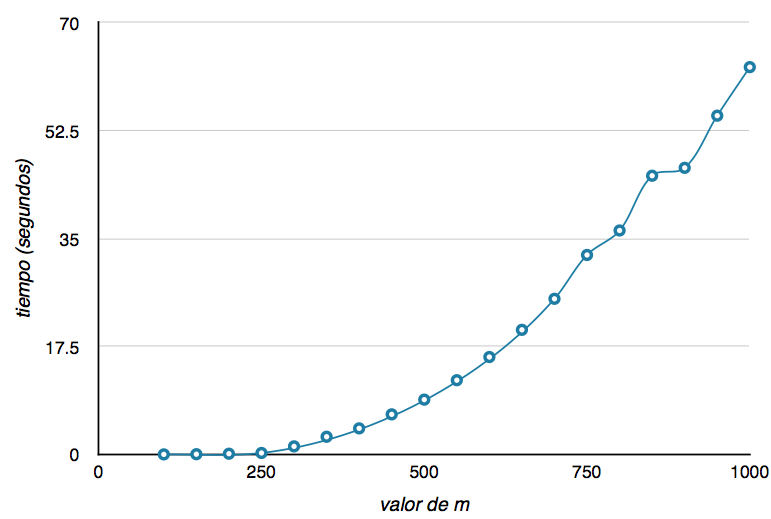
\includegraphics{normal}}%
    }
  	\caption{Multiplicaci\'on est\'andar de matrices}
  	\label{fig:normal}
\end{figure}

\subsubsection{Segunda iteraci\'on}
En el siguiente gr\'afico se representa la complejidad del algoritmo de
multiplicaci\'on de matrices utilizando la estructura de datos \emph{CCS}. Los
ejes representan lo mismo que el gr\'afico anterior.
\begin{figure}[H]
	\centerline{
        \resizebox{0.8\textwidth}{!}{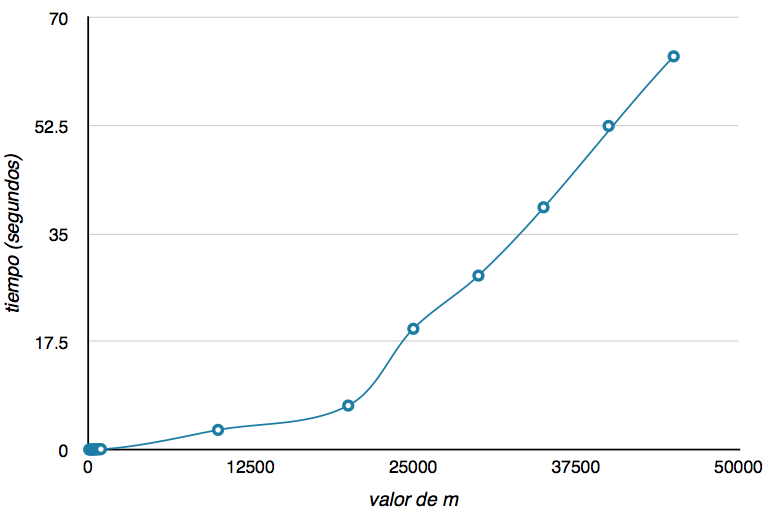
\includegraphics{ccs}}%
    }
  	\caption{Multiplicaci\'on CCS}
  	\label{fig:ccs}
\end{figure}

\subsection{Descripci\'on de los resultados}
\paragraph{}
El resultado m\'as importante que se puede obtener de los gr\'aficos anteriores
es que en el intervalo de hasta 70 segundos, el primer algoritmo puede resolver
hasta matrices de \emph{m = 1000}, mientras que el segundo puede resolver hasta
matrices de \emph{m = 50000} aproximadamente.
Adem\'as, se puede observar que la curva del primer algoritmo crece mucho m\'as
r\'apido que la segunda. Esto puede corresponderse con el hecho de que el
primer algoritmo es de \emph{O(n\textsuperscript{3})}, mientras que el otro es
de orden menor.
\subsubsection{Tercera iteraci\'on}
Si bien se logr\'o optimizar bastante el algoritmo que calcula la matriz A,
mientras se realizaban pruebas se pudo observar un patr\'on en la
construcci\'on de A. Se not\'o que a partir de \emph{m = 3}, la matriz \emph{A}
puede escribirse gen\'ericamente, ya que pequeños bloques de elementos se
repiten a lo largo de la estructura, aumentando la cantidad de bloques
predeciblemente a medida que \emph{m} aumenta. Por lo tanto, se puede evitar tener
que calcular \emph{A} a partir del producto entre \emph{K} y \emph{L}, y en vez
de eso, seguir la siguiente regla para representarla:

\paragraph{}
Cuando \emph{m = 1},
\begin{equation} \label{matrizM1}
A =
\left( \begin{array}{cc}
1 & 0\\
0 & 1\\
\end{array} \right)
\end{equation}
\paragraph{}
Cuando \emph{m = 2},
\begin{equation} \label{matrizM2}
A =
\left( \begin{array}{cccc}
T & Q & R & S\\
R & S & T & Q\\
\end{array} \right)
\end{equation}
\paragraph{}
Cuando \emph{m = 3}, la matriz comienza a expandirse dejando ceros en varias
posiciones. Adem\'as puede verse que el bloque del medio compuesto por \emph{Q,
R, S y T} comienza a repetirse.
\begin{equation} \label{matrizM3}
A =
\left( \begin{array}{cccccc}
T & Q & R & & & S\\
 & S & T & Q & R & \\
R & & & S & T & Q\\
\end{array} \right)
\end{equation}
\paragraph{}
Entonces, para \emph{m \textgreater = 3}, la matriz puede escribirse de forma
gen\'erica de la siguiente forma:

\begin{equation} \label{matrizM4}
A =
\left( \begin{array}{cccccccccccc}
T & Q & R &   &   &  &  &  &  &  &  & S\\
  & S & T & Q & R &  &  &  &  &  &  &  \\
  &   &   & S & T & \ddots&  &  &  &  &  &  \\
  &   &   &   &   &  & \ddots&  &  &  &  &  \\
  &   &   &   &   &  &  & Q & R &  &  &  \\
  &   &   &   &   &  &  & S & T & Q & R &  \\
R &   &   &   &   &  &  &   &   & S & T & Q\\
\end{array} \right)
\end{equation}
\paragraph{}
Siendo
\begin{equation} \label{matrizQ}
Q =
\left( \begin{array}{cccc}
\sin \alpha \cos \beta\\
\cos \alpha \cos \beta\\
\end{array} \right)
\end{equation}

\begin{equation} \label{matrizR}
R =
\left( \begin{array}{cccc}
\sin \alpha \sin \beta\\
\cos \alpha \sin \beta\\
\end{array} \right)
\end{equation}

\begin{equation} \label{matrizS}
S =
\left( \begin{array}{cccc}
-\cos \alpha \sin \beta\\
\sin \alpha \sin \beta\\
\end{array} \right)
\end{equation}

\begin{equation} \label{matrizT}
T =
\left( \begin{array}{cccc}
\cos \alpha \cos \beta\\
-\sin \alpha \cos \beta\\
\end{array} \right)
\end{equation}

Utilizando esta forma de construcción, se logra generar la matriz A de $m =
100000000$ (cien millones) en al rededor de 10 segundos. Antes de comenzar a
tardar por encima del minuto, la computadora se queda sin memoria RAM (por ejemplo,
al probar con 300 millones, ya el sistema operativo retorn\'o NULL al llamar
a \emph{malloc} para reservar la memoria necesaria).

\newpage
\section{Busqueda de autovalores}
Para calcular los autovalores de la matriz se utilizó el procedimiento
recomendado en ``Matrix Market''. En el mismo, se obtienen los autovalores de la
matriz de $2m \times 2m$, $A = K \cdot L$, calculando los autovalores de las m matrices de
$2 \times 2$. \\

Mediante la función \verb+compareEigenvalueMethods+ se puede comprobar que los $2m$
autovalores de las $m$ matrices de $2 \times 2$ corresponden a una buena
aproximación de los autovalores de la matriz $A$. \\

Para obtener los autovalores de las matrices de $2 \times 2$ se resuelve el polinomio
característico a partir de la fórmula cuadrática:

\begin{equation}
    \lambda_{1,2} = \frac{tr(A) + \sqrt{tr(A)^2 - 4 \cdot det(A)}}{2}
\end{equation}

Como comparación, se obtuvieron los autovalores de la matriz A a partir de la función de octave eig,
y se comprobó que nuestros resultados eran correctos.\\

Utilizando la función \verb+getEigenvalues+, se calculan los autovalores. Debido a que
sólo se deben crear y multiplicar matrices de $2 \times 2$, para luego obtener los
autovalores a partir de un método algebraico, se pueden calcular un gran número
de autovalores en tiempos razonable, como se puede apreciar en la siguiente tabla:\\ \\
\begin{tabular}{|l||l|}
\hline
\multicolumn{2}{|l|}{Multiplicaci\'on est\'andar}\\
\cline{1-2}
\textbf{m}&\textbf{tiempo (seg)}\\
\hline\hline
10 & 0.006 \\
100 & 0.050\\
1000 & 0.304\\
10000 & 2.541\\
100000 & 39.905\\
\hline
\end{tabular}\\ \\

En un principio se intentó utilizar el algoritmo $QR$ para obtener los
autovalores de $A$. Este acercamiento no di\'o resultados, ya que se not\'o que la
matriz no converg\'ia a una forma triangular. En un principio se pens\'o que esto
se deb\'ia a la existencia de autovalores complejos, pero luego se descubri\'o que
la raz\'on era que la matriz $A$ es ortogonal, por lo tanto al descomponer en
matrices $QR$, resulta que $Q$ equivale a $A$, y $R$ a la matriz identidad. Por lo tanto, se opt\'o por
calcular los autovalores de las matrices de $2 \times 2$.\\

La matriz $A$ que se obtiene de multiplicar $K$ por $L$ es rala, especialmente para
valores grandes de $m$. Debido a esto, el algoritmo $QR$, de haber funcionado,
habr\'ia sido muy ineficiente para calcular los autovalores. En un principio, se
pens\'o en utilizar el M\'etodo de Arnoldi. Este procedimiento iterativo para
matrices ralas, va generando a partir de $A$ una matriz de Hessenberg. Una
fracci\'on de los autovalores de esta matriz son una buena aproximaci\'on a los
autovalores de $A$. Adicionalmente, el algoritmo $QR$ corre mucho m\'as
eficientemente sobre matrices de Hessenberg, por lo tanto, el M\'etodo de
Arnoldi, da la posibilidad de conseguir un conjunto de autovalores de $A$ de
manera eficiente. \\
\newpage
\section{Conclusiones}
La matriz A del modelo de Ising representa un buen ejemplo de la importancia de
la correcta elecci\'on de una estructura de datos adecuada, y algoritmos
eficientes a la hora de resolver un problema.\\
No solo esto, sino c\'omo, probando propiedades o caracter\'isticas del
problema en cuesti\'on matem\'aticamente, es posible evitar cálculos
redundantes y optimizar aun m\'as un programa, dando tres diferentes aristas de
gran relevancia por las cuales uno puede aproximarse a una soluci\'on \'optima.\\
Esto tambi\'en se pudo apreciar en el c\'alculo de los autovalores, donde el
algoritmo final utilizado ni siquiera necesit\'o de la construcci\'on de A para
poder calcular sus autovalores.

\paragraph{}
\newpage
\section{Bibliograf\'ia}
Watkins, David S., Fundamentals of Matrix Computations. New York: John Wiley \&
Sons, Inc., 2002\\
Yousef, Saad, Numerical Methods For Large Eigenvalue Problems. Society for
Industrial and Applied Mathematics, 2011\\
Gene H. Golub \& Charles F. Van Loan, Matrix computations, The Johns Hopkins
University Press, Baltimore, 1996\\
\url{http://en.wikipedia.org/wiki/Sparse_matrix}
\url{http://netlib.org/linalg/html_templates/node91.html#SECTION00931100000000000000}
\url{http://netlib.org/linalg/html_templates/node92.html#SECTION00931200000000000000}
\end{document}
